\section{Metodología Propuesta: IA para Optimización Autónoma}

\subsection{4.1. Arquitectura del Agente DRL}

Aunque los agentes de reinforcement learning individuales han mostrado potencial, la naturaleza distribuida y acoplada de las NTN exige un enfoque multi-agente desde el principio. Nuestra arquitectura considera cada satélite como un agente inteligente que toma decisiones de forma parcialmente descentralizada mientras comparte información limitada con vecinos a través de ISL.

Particularmente llamativo es el diseño híbrido que combina elementos colaborativos propuestos por Cao et al. \cite{Cao2023} con capacidades avanzadas de beam management. Cada agente observa un estado local enriquecido que incluye canales estimados de sus usuarios servidos, niveles de interferencia percibida y demandas de tráfico. El espacio de acciones abarca asignación discreta de potencia por beam, partición de ancho de banda y orientación fina de beams.

Mohsin et al. \cite{Mohsin2025} demuestran la utilidad de DRL en entornos con RIS activos para mitigar interferencias; extendemos esta idea permitiendo que los agentes ajusten dinámicamente patrones de beamforming para explotar tanto ganancia direccional como posibles reflexiones constructivas en escenarios TN-NTN integrados. 

El agente emplea una arquitectura actor-critic con redes neuronales profundas compartidas parcialmente entre satélites para acelerar el aprendizaje inicial, manteniendo al mismo tiempo especialización local ante condiciones orbitales distintas.

\subsection{4.2. Guía por Large AI Models}

Uno de los cuellos de botella más persistentes en aplicaciones DRL puras radica en la ineficiencia del entrenamiento en espacios de acción y estado de alta dimensionalidad. Aquí es donde la integración de Large Artificial Intelligence Models (LAM) marca una diferencia sustancial.

Inspirados en el framework presentado por Ibrahim et al. \cite{Ibrahim2026}, incorporamos un LAM como módulo de razonamiento de alto nivel que actúa como guía semántica y generador de conocimiento previo. Este modelo procesa descripciones textuales del estado actual del sistema —posiciones orbitales, patrones de tráfico, métricas de rendimiento recientes— y produce sugerencias estratégicas, prioridades de objetivos y explicaciones naturales que enriquecen el proceso de reward shaping.

Resulta revelador observar cómo esta guía no solo acelera la convergencia sino que mejora notablemente la interpretabilidad de las políticas aprendidas. El LAM inyecta atención contextual sobre trade-offs críticos (por ejemplo, priorizar usuarios en cell-edge versus minimizar interferencia global), modulando los pesos dinámicos en la función de reward. De esta forma, el agente DRL no opera como una caja negra completa, sino que recibe retroalimentación de alto nivel que alinea sus decisiones con objetivos del operador de red.

Lejos de ser un mero wrapper, esta integración bidireccional permite que el LAM refine sus sugerencias con base en el rendimiento observado a lo largo de episodios de entrenamiento.

\begin{figure}[h]
\centering
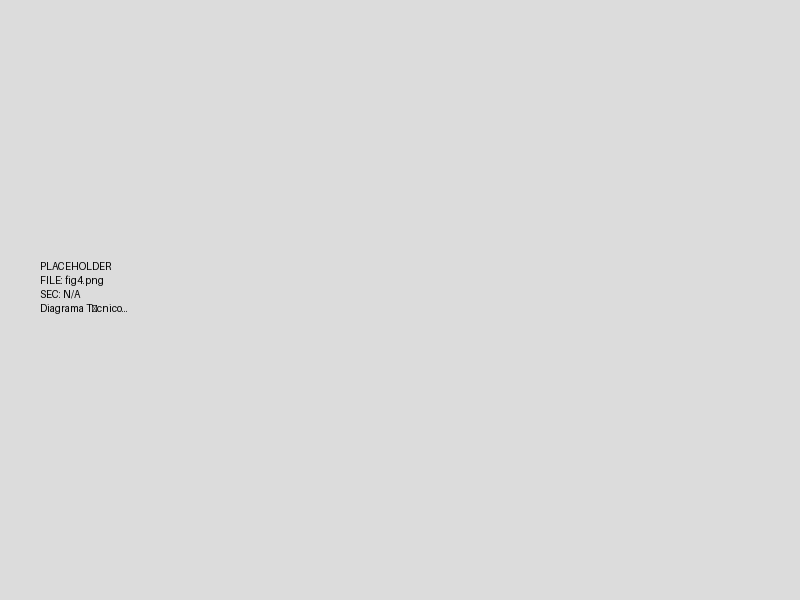
\includegraphics[width=\linewidth]{fig4.png}
\caption{Diagrama del framework propuesto de optimización autónoma NTN: agentes DRL multi-satélite guiados por LAM, con módulo LSTM de predicción de canal y bucle de interacción con el entorno NTN.}
\label{fig:framework_propuesto}
\end{figure}

\subsection{4.3. Algoritmos de Entrenamiento y Predicción LSTM}

Ningún esquema de optimización en NTN puede ignorar la necesidad de anticipación. Siguiendo la línea de Minani et al. \cite{Minani2025_Channel}, integramos un predictor basado en LSTM que estima el estado del canal en los próximos 5-10 slots temporales utilizando secuencias históricas de mediciones CSI, posiciones relativas y ángulos de elevación.

Este predictor alimenta al agente DRL, transformando el problema de observación parcial en uno semi-predictivo. El entrenamiento completo sigue un esquema de actor-critic con experiencia replay priorizada y actualizaciones soft de los parámetros target.

\begin{algorithm}[h]
\caption{Entrenamiento del Framework LAM-DRL para NTN}
\label{alg:entrenamiento}
\begin{algorithmic}[1]
\State Inicializar redes actor y critic, buffer de replay y LAM
\For{episodio = 1 to $M$}
    \State Obtener estado inicial $s_0$ del simulador NTN
    \For{t = 1 to $T$}
        \State Predecir canal futuro con LSTM
        \State Generar guía semántica vía LAM dado $s_t$
        \State Seleccionar acción $a_t \sim \pi_{\theta}(a|s_t, g_{LAM})$
        \State Ejecutar acción, observar $r_t$, $s_{t+1}$
        \State Almacenar transición y actualizar pesos con reward shaping guiado
    \EndFor
    \State Actualizar LAM con trazas de rendimiento
\EndFor
\end{algorithmic}
\end{algorithm}

Este pseudocódigo resume el flujo principal. Cabe matizar que el entrenamiento se realiza principalmente en simulador con transferencia posterior al entorno real (sim-to-real), técnica esencial dada la imposibilidad de exploración exhaustiva en sistemas satelitales operativos. La combinación de predicción LSTM, guía LAM y ejecución multi-agente DRL permite alcanzar adaptabilidad en tiempo real manteniendo robustez ante variaciones no vistas, superando limitaciones identificadas en trabajos previos.

En conjunto, el framework propuesto representa un paso concreto hacia la automatización inteligente de enlaces NTN, donde la inteligencia artificial no solo optimiza recursos sino que razona sobre las consecuencias de sus decisiones a múltiples escalas temporales.